%Exp 1-3
\chapter{Velocity, Acceleration, and $g$} \label{chap:velocity}
\section{Introduction}

In this experiment you will study motion with constant velocity and motion with constant acceleration.  Ordinarily, it is difficult to examine these kinds of motion with precision, since objects in free fall tend to move too rapidly, and frictional forces arise in most everyday situations.  These factors hinder a direct observation of the underlying physical principles of motion, and in fact this is one of the reasons why these principles were poorly understood until Galileo's famous experiments.  In this lab, it will be possible to study motion in the absence of almost any friction by using a rider on an air-track.  The air-track has rows of small air jets running down its side, which support the rider on a thin film of air and allow it to float just above the track -- minimizing contact and thereby minimizing friction.  When the track is level and the rider is given a slight push, it will move with constant velocity; when the track is slightly inclined, the rider will experience a small acceleration due to the component of gravity which is parallel to the track. \myskip

To study the motion of the rider, you need to be able to make accurate measurements of its position at given intervals of time.  This is done using a sonar device called the \textbf{Sonic Ranger}. This apparatus sends out discrete pulses of sound waves, which are reflected back by the object or objects in its path. The \textbf{Sonic Ranger} is in turn connected to a computer, which calculates the distance to the object based on the time it takes the signal to leave the sonar module and return.  If a series of such measurements is made in rapid succession, then the computer can reconstruct the motion of the rider over some time interval, and this information can be used for other calculations, such as the ``instantaneous'' velocity or acceleration of the rider as a function of time.  An essential part of this lab is becoming familiar with using the computer to obtain and analyze data.  The computer offers many extraordinary advantages over manipulating data by hand, but you can benefit from it only if you have learned how to use it effectively and understand its limitations.

\begin{figure}[h]
    \begin{center}
        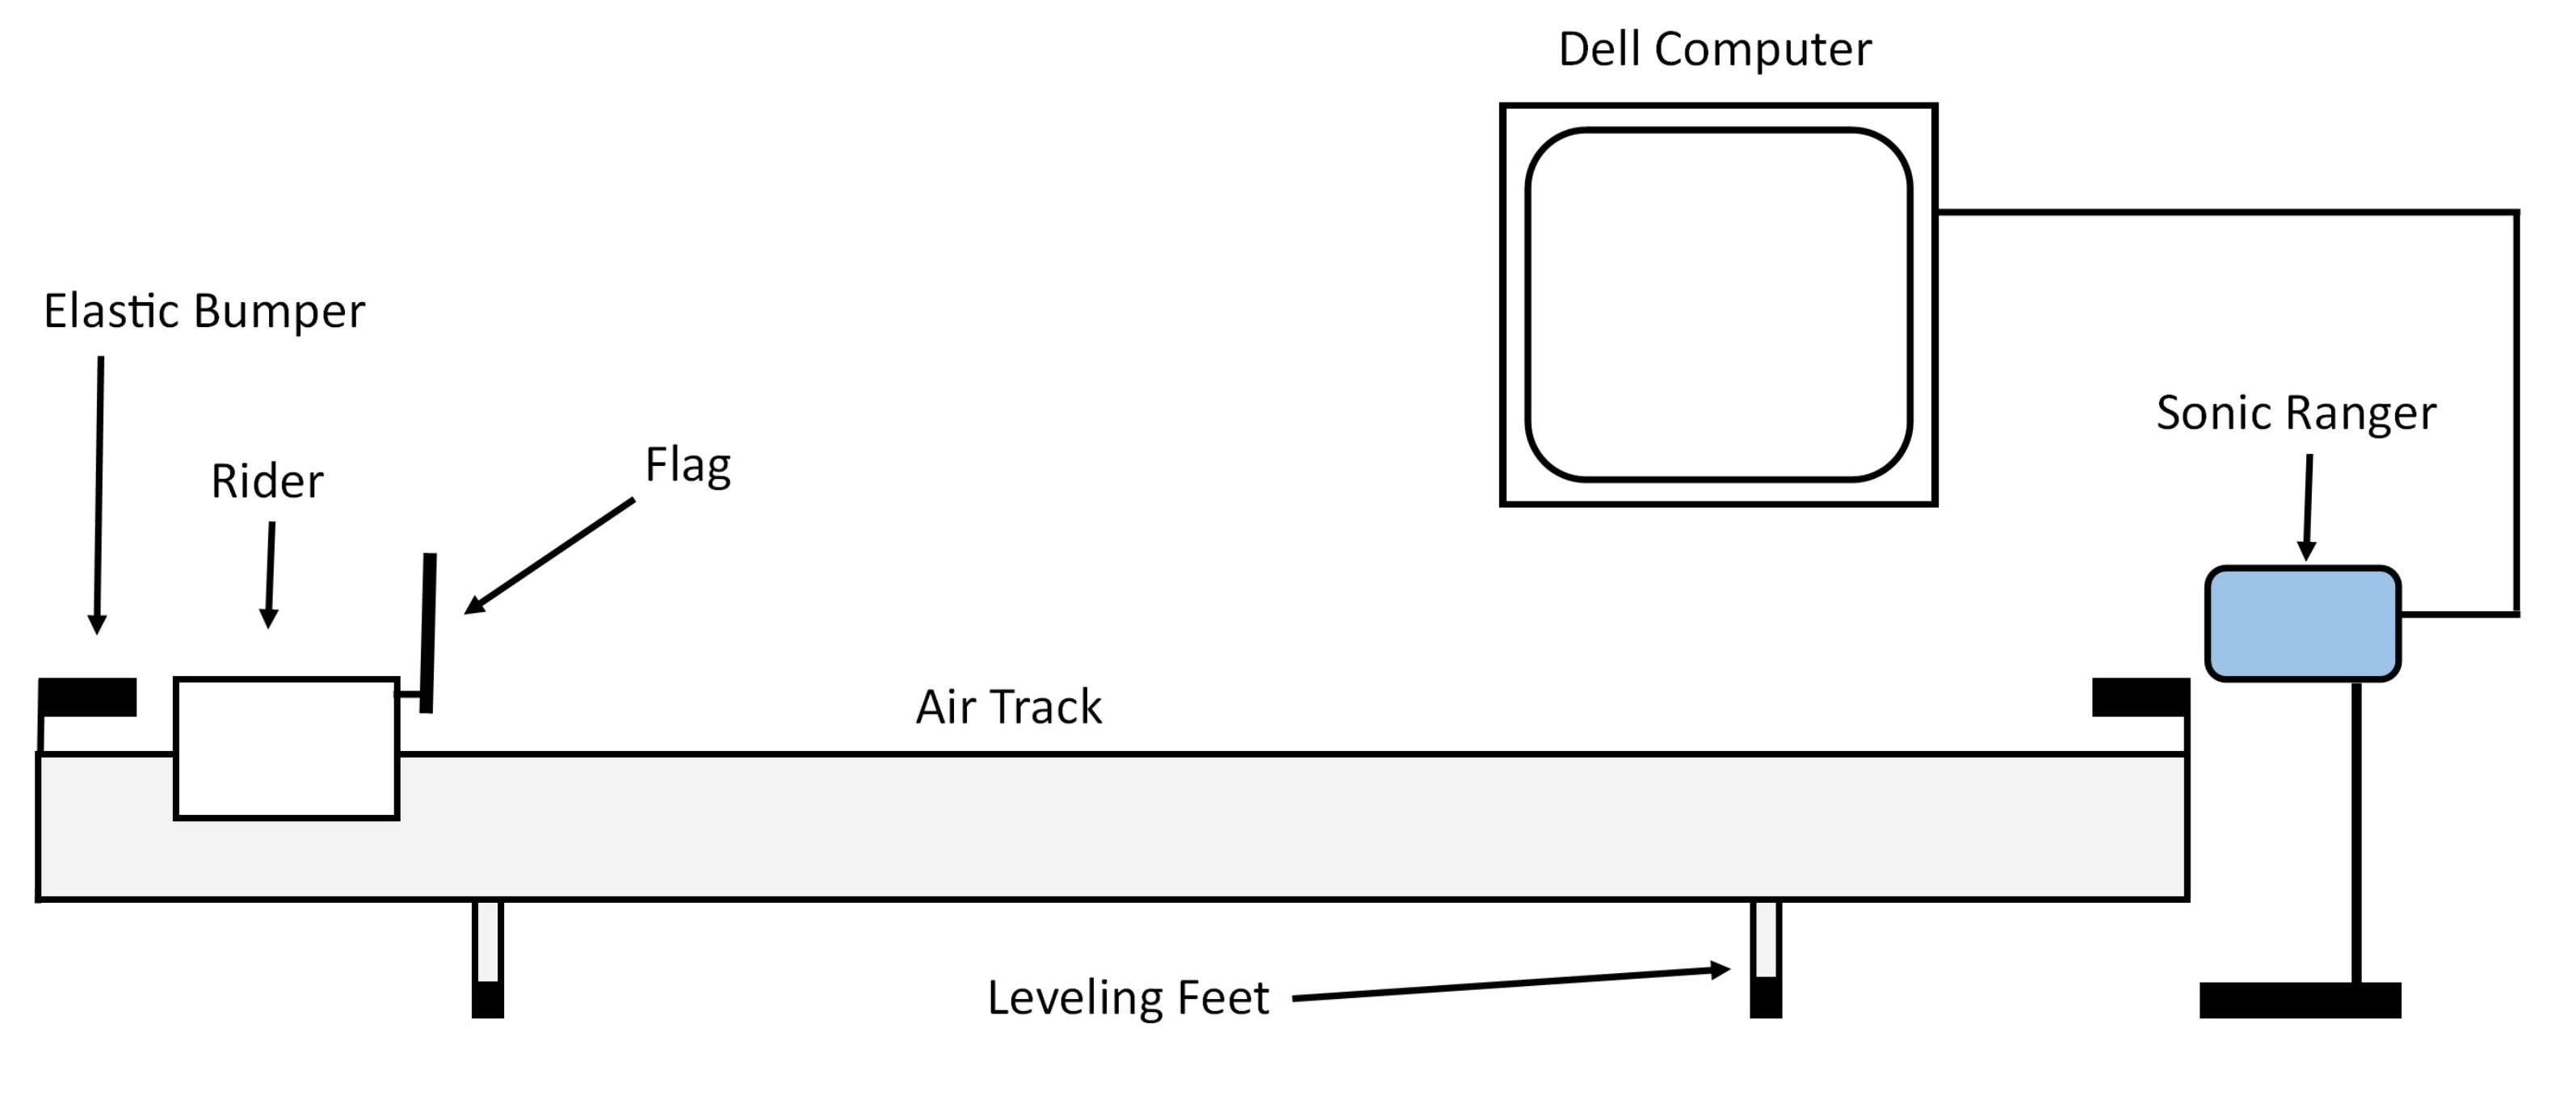
\includegraphics[width=0.9\textwidth]{./Exp1-3/pic/image11.jpg}
    \end{center}
    \caption{Schematic Diagram of the Air Track}
    \label{fig:airtrack}
\end{figure}

\section{Set-up}

\subsection{Getting Started}

Some of the laboratory computers require you to log on before you can view and use the desktop screen.  To log on, use the user name \textbf{student} and the password \textbf{student}.  When the desktop screen is visible, double click on the VELOCITYLAB icon to load the Sonic Ranger software.  (In this lab, all mouse clicks use the left button.)  The screen shown in Figure \ref{fig:velocitylab}, with two empty graphs displayed, should now appear.  The computer is now ready to take data.  The top graph will show position (meters) versus time (seconds), while the bottom graph will show velocity (meters/second) versus time (seconds).
\begin{figure}[h]
    \begin{center}
        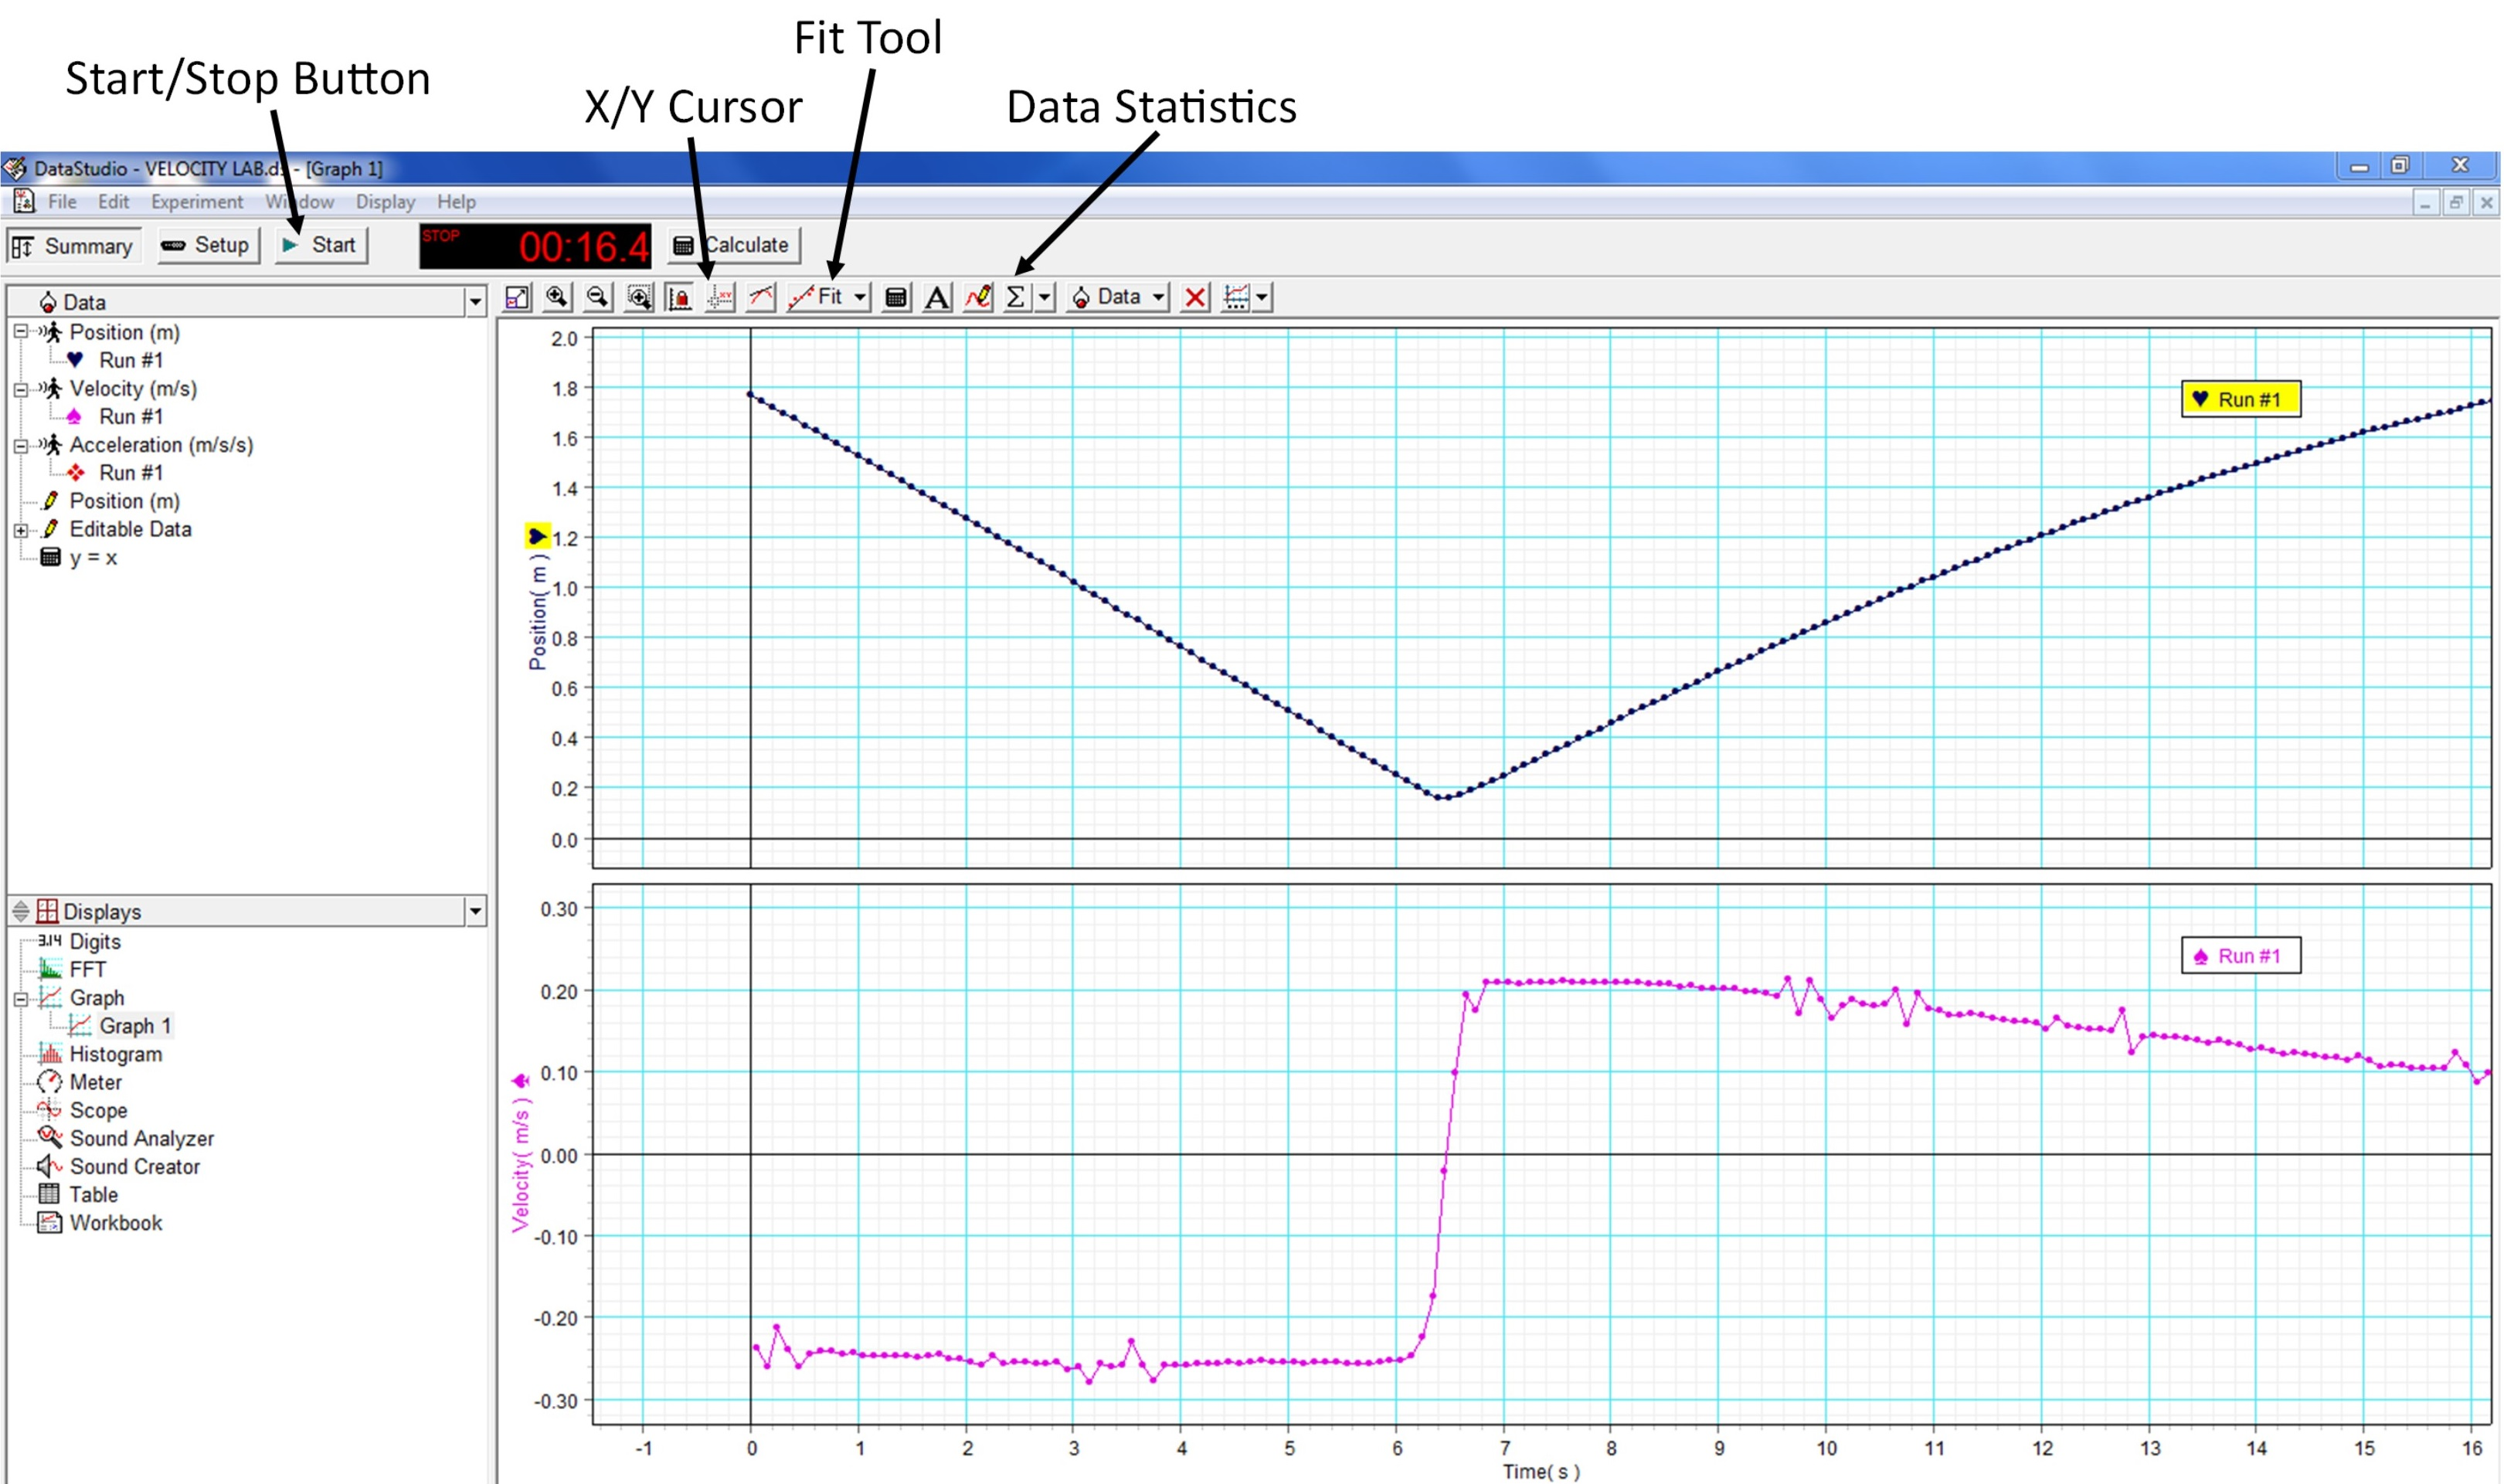
\includegraphics[width=1.0\textwidth]{./Exp1-3/pic/image16.jpg}
    \end{center}
    \caption{VELOCITYLAB User Interface}
    \label{fig:velocitylab}
\end{figure}

To begin taking data, single click on the screen's \textbf{Start} button. As the data are being collected, both graphs will display the measurements. To stop taking data, single click on the screen's \textbf{Stop} button (the button that replaced the Start button). After analyzing the graphs, you can erase the data and begin collecting new data by single clicking on the \textbf{Start} button. \myskip

Note that the position, velocity, and time axes will automatically rescale so that all of the data points are visible on the graphs.  To change a graph scale manually, just click and drag any number on the appropriate axis.  Clicking and dragging the axis line will move the axis in the display window.  Notice that the time axes of both graphs will rescale and move together so that the time axes of the position and velocity graphs are always aligned. \myskip

Remember, after finishing your experiment, to reset your display settings to their original default values.  To do this, simply quit the program by single clicking on the pull-down \textbf{File} menu and then choosing the \textbf{Quit} option.  A dialog box will ask if you want to save the activity.  Choose the \textbf{No} option and the screen will return to the desktop display.  (You cannot save the activity, and choosing the \textbf{Yes} option or the \textbf{Cancel} option will just make the dialog box disappear without closing the program.)  You can double click on the desktop's VELOCITYLAB icon to restart the program.  You may follow this procedure whenever you want to clear the screen and return to the original default settings.

The Sonic Ranger measures and records the position of an object every 0.05 seconds.  The graph of position versus time is then obtained directly from these position measurements.  The software constructs the graph of velocity versus time by calculating the average velocity (the change in distance divided by the time interval) based on the successive position measurements.  Since the position measurements are taken very closely together, the calculated average velocity for each interval is reasonably close to the instantaneous velocity at any instant within that interval. \myskip

The Sonic Ranger has two modes of operation, which are controlled by the switch on top of the Sonic Ranger module.  Move the switch to the person icon to take good-quality data from a large object (such as a moving person) using a wide sonar beam.  Move the switch to the cart icon to take good-quality data from a small object (such as a rider moving on an air track) using a narrowly focused sonar beam. \myskip


\subsection{Setting Up the Sonic Ranger for Use with the Air Track}

\textbf{Note}: It is important that you take care when using the rider and air-track.  Don't let the rider sit on the track when the air is off, and don't let the flag-side of the rider collide with the elastic bumper. Both of these can cause the rider and air-track to scrape against each other, leaving scratches which permanently damage the equipment. \myskip

Set the Sonic Ranger just at the right end of the track, and switch the Sonic Ranger to the cart mode.  Adjust the location and tilt of the device so that the sonar beam travels horizontally along the center line of the air track.  This will allow you to make sure the Sonic Ranger is able to detect the rider when it is at the far end.  Turn on the air for the air-track and set the rider at the far left end of the track.   Prop up the right side of the track so that the rider stays at the left end. Follow the procedure mentioned in the previous section to collect data.  The distance from the Sonic Ranger to the flag on the rider will be approximately $1.8\,\mathrm{m}$, so if it is aimed correctly you should see a stationary object about $1.8\,\mathrm{m}$ away on the graph. If not, try to re-aim it while you are taking data or try taking data again.  You can then check the alignment more precisely by giving the rider a small push along the air-track, and observe whether the computer plots the rider's position smoothly throughout the length of the track.  If there are ``static-like'' jumps in the plot, then the sound waves are not reflecting properly back to the Sonic Ranger, and you will need to align it more carefully.

\subsection{A Note about Distances}

The Sonic Ranger is unable to detect objects that are too close, because it requires a certain amount of time between sending and receiving signals.  Close objects will reflect signals too early for the Ranger to interpret the data correctly.  Therefore, always work with distances greater than $20\,\mathrm{cm}$ from the Sonic Ranger to insure that the distance to the object is determined correctly. \myskip

Note also that the scale on the air-track increases as you read toward the right.  Since the Sonic Ranger is aimed left, its scale increases toward the left, with the origin at the faceplate of the module, not the right end of the track (see Figure \ref{fig:measurement}).  It is extremely important that you keep these two scales separate in your work.  You should use the readings from the Sonic Ranger (which the computer indicates in meters) for all of your experimental calculations, and use the scale on the air-track (which is marked in centimeters) only for positioning the rider in the same place when you are repeating an experiment over several trials.
\begin{figure}[h]
    \begin{center}
        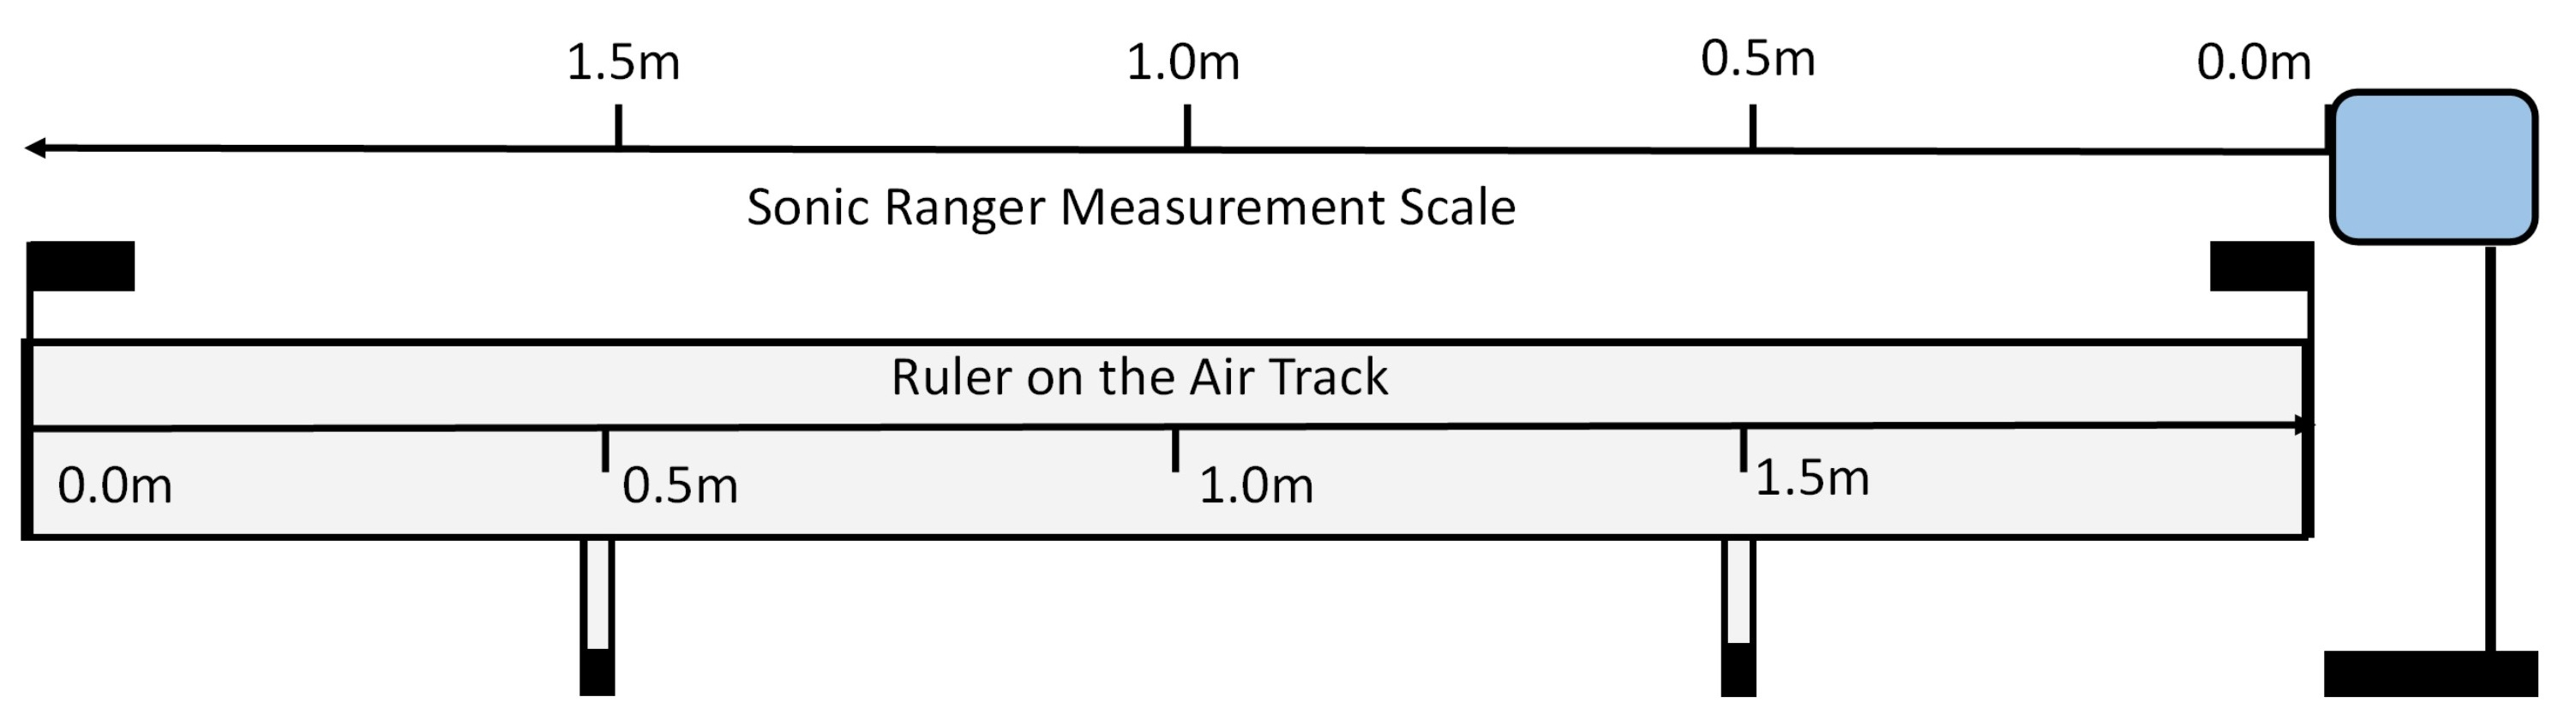
\includegraphics[width=0.9\textwidth]{./Exp1-3/pic/image12.jpg}
    \end{center}
    \caption{The measurement scale of the Sonic Ranger starts at its faceplate, and increases toward the left, \emph{oppositely of the ruler on the air track}}
    \label{fig:measurement}
\end{figure}

\section{Motion with Constant Velocity}

\subsection{Leveling the Air Track}

To study motion with constant velocity it will be necessary to level the air-track as carefully as possible so that the rider does not tend to accelerate in one direction.  The left side of the air-track has two adjustable feet; the right foot is not adjustable, but you may raise it by stacking sheets of paper beneath it.  (Avoid using the metal shims for leveling the track, since you will be using them later to raise it to a fixed inclination.)  The air-track has been machined to remain extremely straight along its entire length, but because the rider is also extremely sensitive to the slightest variation along the track, you will find that the rider sometimes remains stationary in one region of the track but tends to drift when it is in another region.  It is not always possible to completely level the track, but you should try to minimize these irregularities by making sure that the drift is as small as possible in most parts of the track, and that the direction of the drifts are more or less random.  (If all the drifts tend in the same direction, then this indicates that you can make the track more level.)

\subsection{Taking Data}

Once you are satisfied that the track is sufficiently level, set the rider at the $150\,\mathrm{cm}$ mark.  Begin collecting data, and then give the rider a gentle push toward the left.  Make sure that you are able to take data over a substantial portion of the return trip after it has bounced off the elastic bumper at the left end, and also make sure that the position data is smooth and without jumps.

\begin{itemize}
    \item Is the velocity graph reasonable?  The time scales of the two graphs are always the same, so you should be able to see how the rate of change in the displacement graph corresponds to the velocity.
\end{itemize}

\subsection{The Coefficient of Restitution}

When two objects collide and bounce away from each other, they tend to lose some of their energy in the collision, and the rebound velocity between the two objects is therefore less than the initial velocity between them.  This is why objects that are dropped will sooner or later stop bouncing.  The elasticity of the collision can be indicated by $e$, the \textbf{coefficient of restitution}, which is defined as the speed after the collision divided by the speed before the collision:
\begin{equation}
    e = \left|v_f/v_i\right|
\end{equation}

A perfectly elastic collision, one in which no energy is lost, would therefore have a coefficient of restitution equal to one; an elastic ``super'' ball is a good example of an object whose coefficient of restitution in many collisions is often close to one.  You can calculate $e$ for the case of the rider colliding with the elastic bumper by using the data you collected in this experiment.

\subsection{Using the Smart Tool to Read off Data Points}

To use the Smart Tool in one of the graphs; select a graph (position or velocity) by clicking in the first quadrant of the graph and then clicking on the menu's Smart Tool button (this is labeled as `xy cursor' in figure \ref{fig:measurement}.  This will activate crosshairs that can be used to select a data point and display its coordinate data pair.  As you get closer to a data point, the Smart Tool will ``gravitate'' toward that data point.  To change the position of the crosshairs of the Smart Tool, move the cursor over the center of the Smart Tool until the pointer turns into two crossed double arrowheads and a hand.  Drag the cross hairs of the Smart Tool to the desired location.  To deactivate the Smart Tool in a graph that has been selected, just click the Smart Tool menu button again.  \myskip

Note that if you activate the Smart Tool in the second graph before the Smart Tool has been deactivated in the first graph, cross hairs will appear in both graphs simultaneously and can be moved together along the common time axis.

\subsection{Determining the Coefficient of Restitution}

You should calculate $e$ from the data just collected using two different methods. \myskip
\begin{itemize}
\item In the first method, use the position versus time graph with the Smart Tool to read off and record the $(t,x)$ coordinates of 5 reasonably separated points before the bumper collision and 5 reasonably separated points after the collision.  Choose representative points that are not part of extraneous effects (which occur at the ends of the motion, in the small region of the collision, and at irregularities in the air track itself).
\begin{enumerate}
\item In Microsoft Excel, plot the 5 $(t,x)$ data points and determine a line of best fit. Be sure to plot error bars on both axes (error bars on the time axis can be found using the precision of the Sonic Ranger ($0.05 s$) and error bars on the position axis can be found using the precision of the Sonic Ranger ($0.01 m$).
\item Determine the initial velocity from the slope of your best-fit line with uncertainty. Uncertainty in initial velocity can be found by propagating the uncertainties in the slope of your best-fit line.
\item    Repeat steps 1-2 for the 5 points after the collision and determine the final velocity with uncertainty.
    \item Calculate $e$ from the ratio of the two velocities with uncertainty found by propagating uncertainties in initial velocity $v_i$ and final velocity $v_f$.
\end{enumerate}

\item In the second method, use the velocity versus time graph with the Smart Tool to read off and record the velocity values for 5 reasonably separated points before the collision and 5 reasonably separated points after the collision.  Once again, choose representative points that are not part of extraneous effects. Perform the analysis in Microsoft Excel.
\begin{enumerate}
\item Calculate the initial velocity $v_i$ by averaging your 5 chosen initial velocity data points. Include uncertainty in average initial velocity using the 2/3 method.
\item Calculate the final velocity $v_f$ by averaging your 5 chosen final velocity data points. Include uncertainty in average final velocity using the 2/3 method.
    \item Calculate $e$ from the ratio of these two average values with error by propagating uncertainties in initial velocity $v_i$ and final velocity $v_f$.
        \end{enumerate}
    \item Which method  gives a more {\it{accurate}} value for $e$ (think about what the value of $e$ {\it{should}} be)?
    \item Which method gives a more {\it{precise}} value for $e$ (think about the difference between {\it{precision}} and {\it{accuracy}})?
\end{itemize}
\section{Gravitational Acceleration}

A small constant force can be applied to the rider by inclining the track slightly.  The component of gravity which acts on the rider parallel to the air-track is equal to $g\sin(\theta)$ as indicated in Figure \ref{fig:slope}.

\begin{figure}[h]
    \begin{center}
        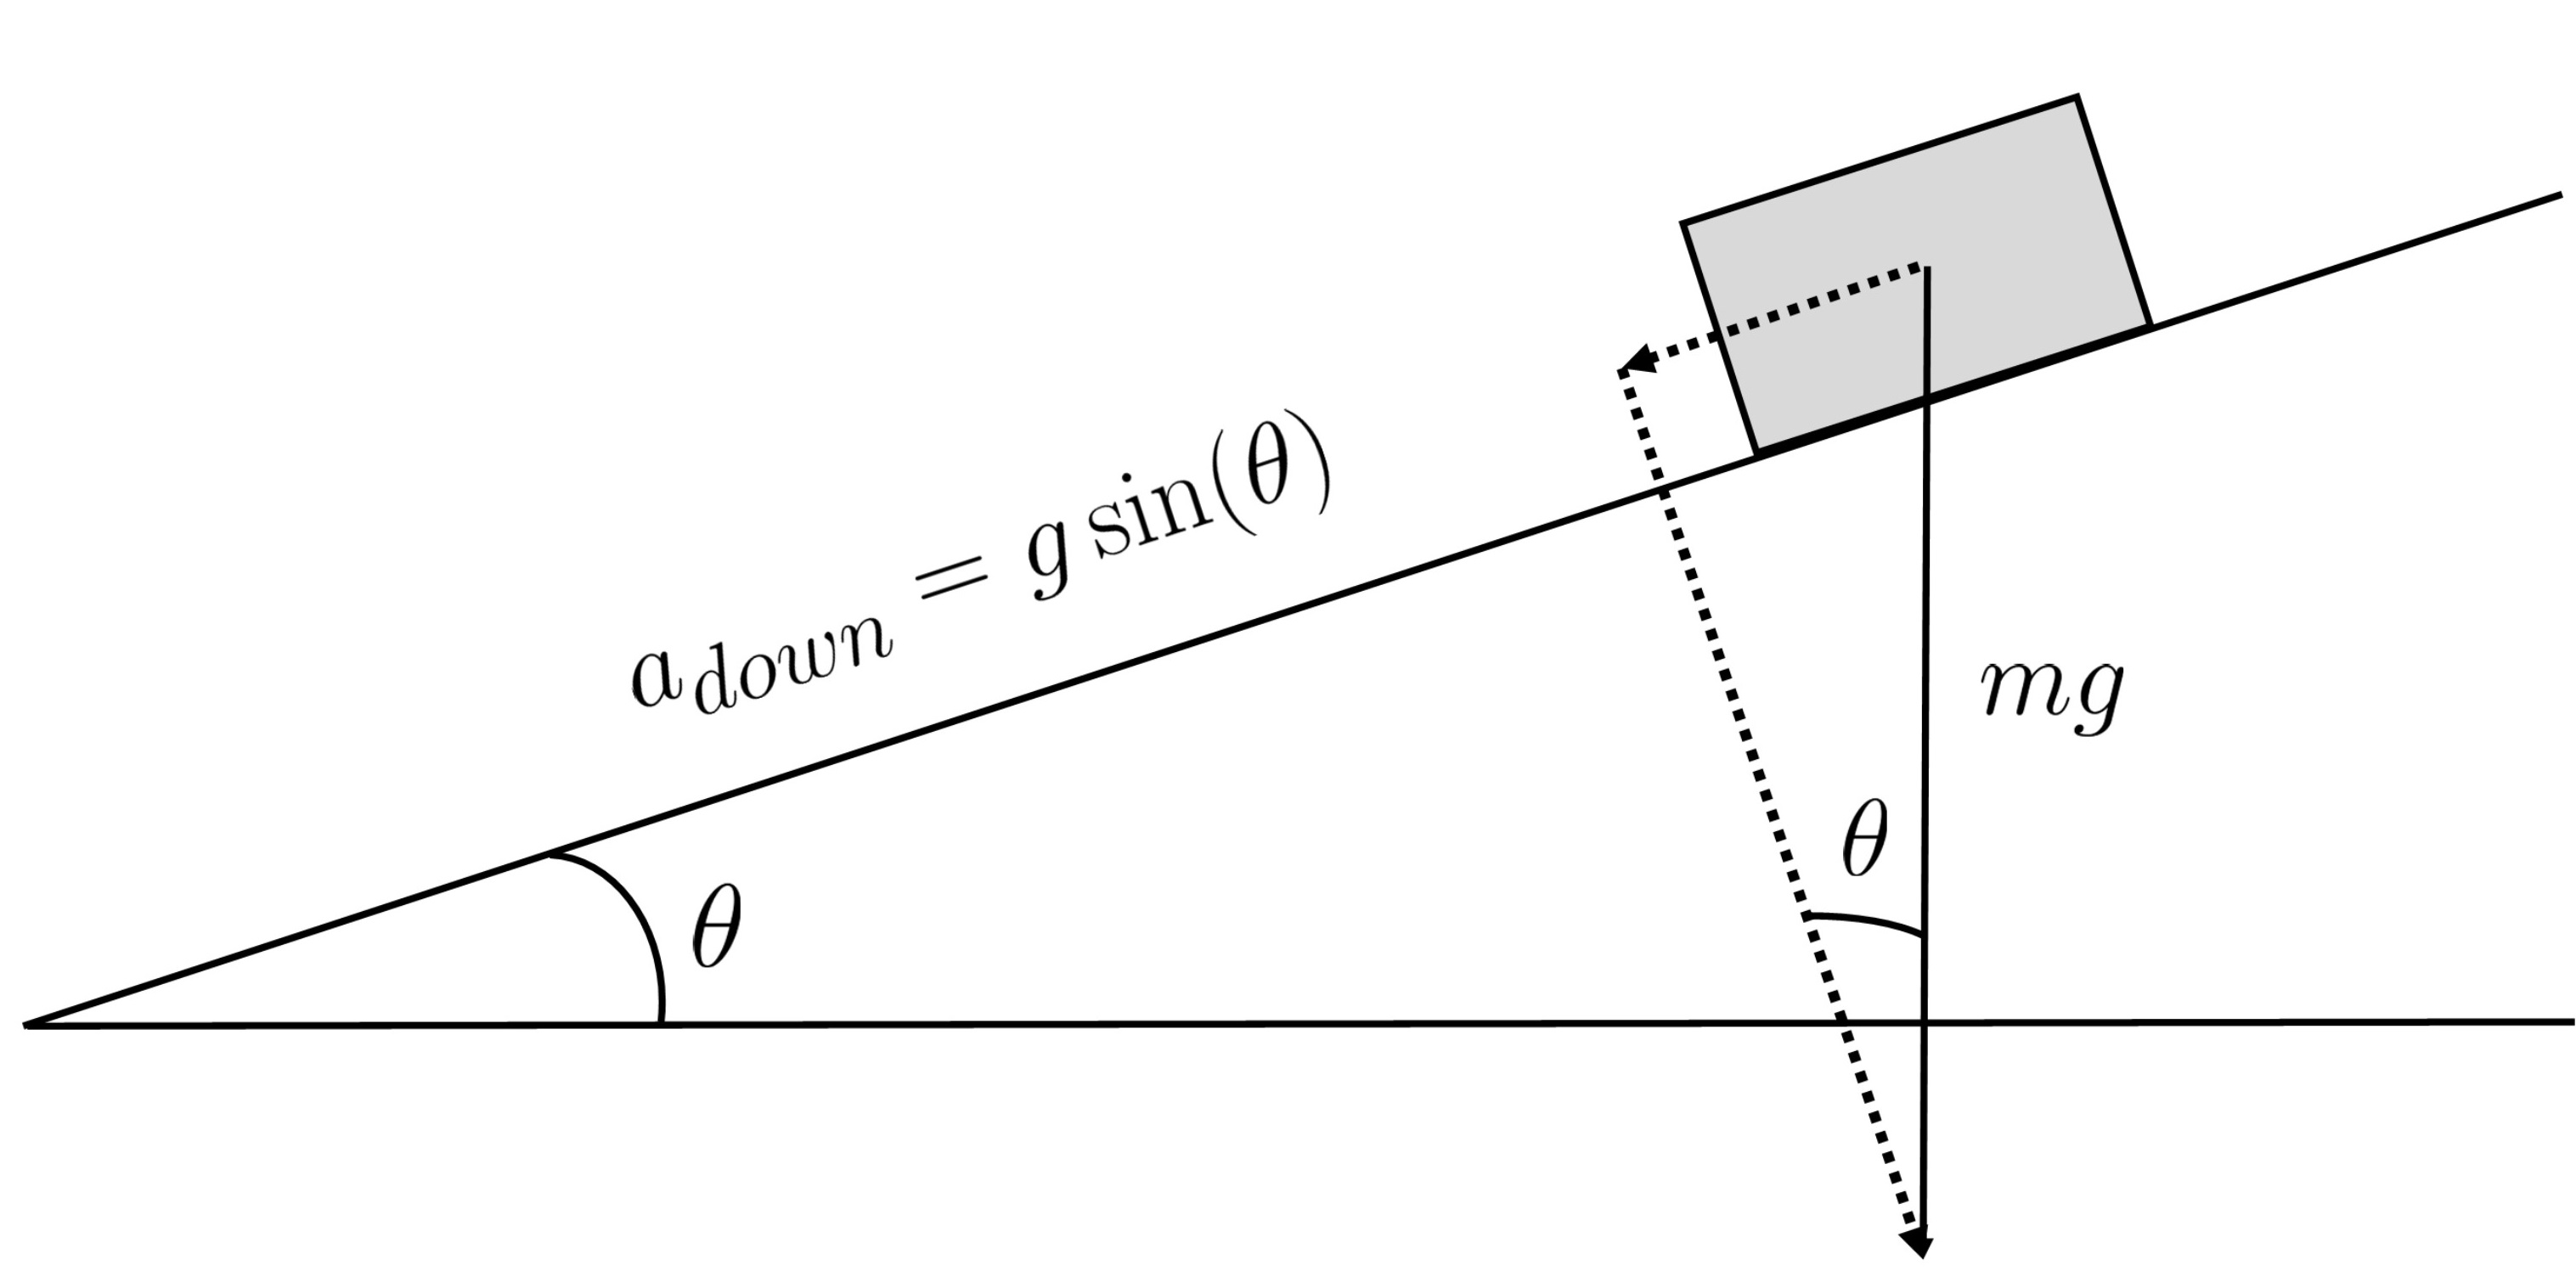
\includegraphics[width=0.8\textwidth]{./Exp1-3/pic/image14.jpg}
    \end{center}
    \caption{Gravitational Acceleration}
    \label{fig:slope}
\end{figure}

Use a few of the shims provided to elevate the right side of the air-track. NOTE: All of the shims are $1.24\,\mathrm{mm}$ thick. \myskip

It is important to remark in the small angle approximation, $\sin\theta \sim \tan(\theta) \sim h/D$, where $D$ is the horizontal distance between the two leg supports. In our case, $D=1.0m$, so $\sin(\theta) \sim h$ (see Figure \ref{fig:shims}). And so, {\it{ $\sin\theta$ is equal to the height of the shims in meters}}.
\begin{figure}[h]
    \begin{center}
        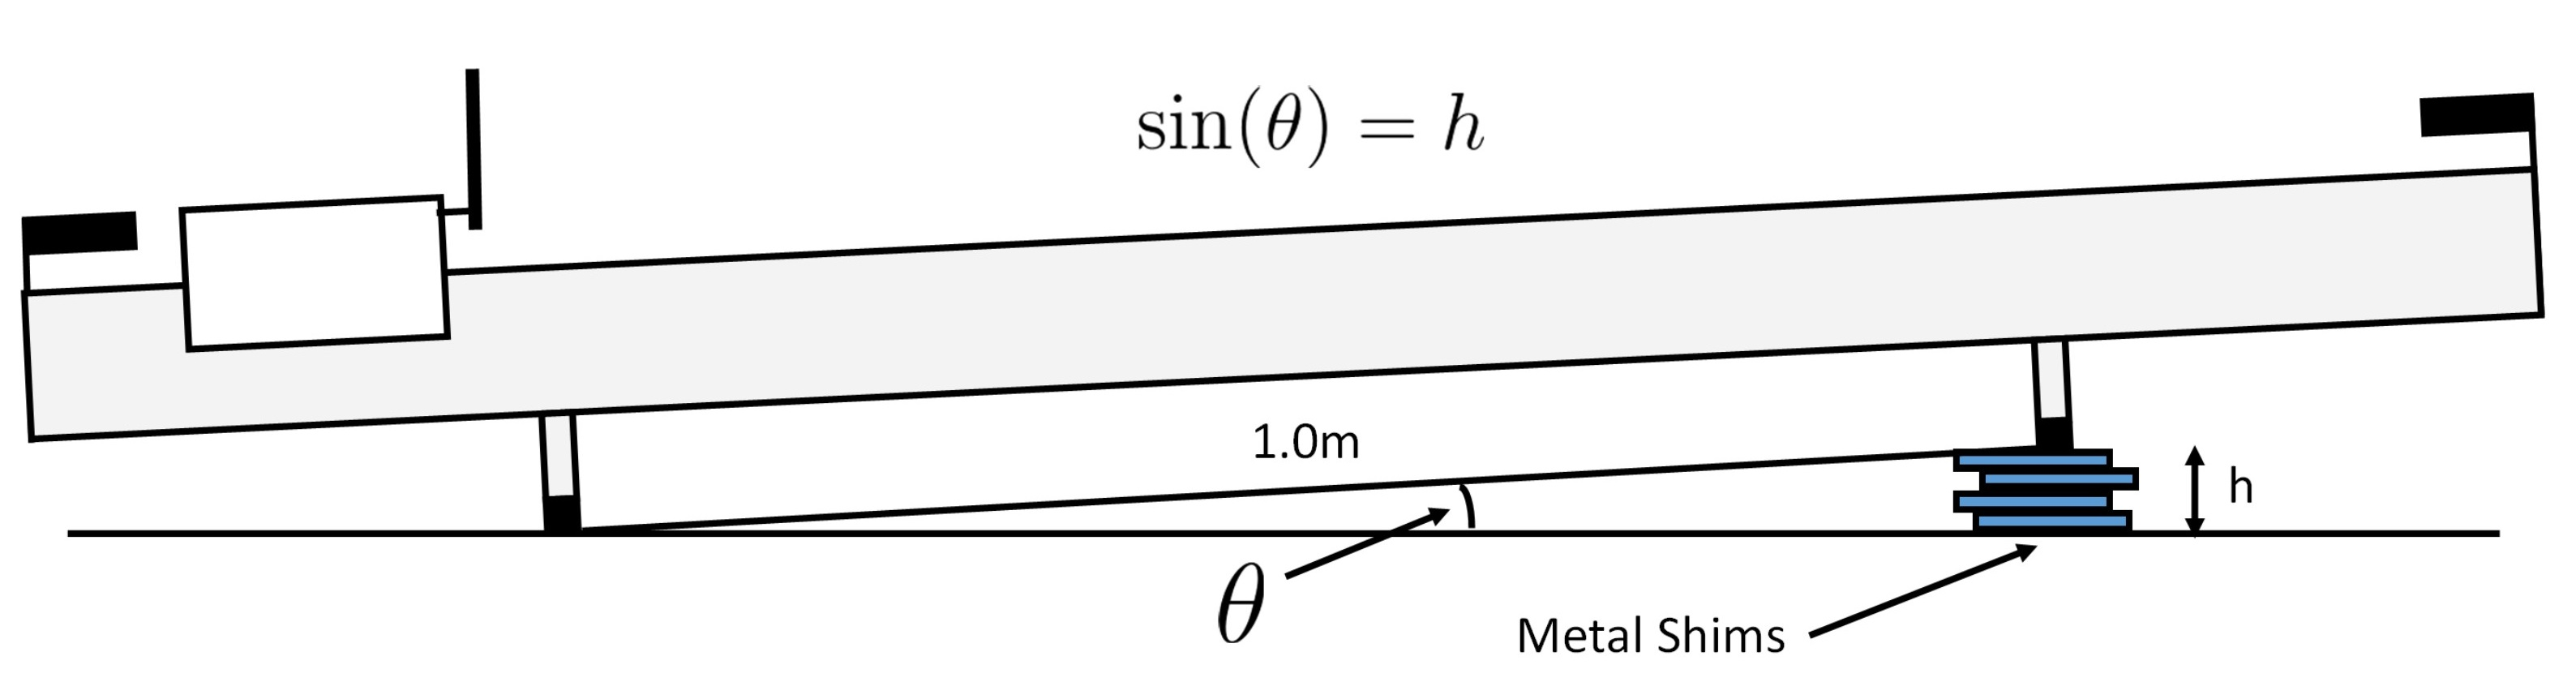
\includegraphics[width=0.8\textwidth]{./Exp1-3/pic/image15.jpg}
    \end{center}
    \caption{Tilting the Air Track}
    \label{fig:shims}
\end{figure}

A convenient method for taking data is as follows.  Set the rider on the air track at a given point, say at the $150\,\mathrm{cm}$ mark, and release it.  Start taking data and record the motion as the rider goes down the track, bounces off the elastic bumper, goes back up the track, and then heads back down the track. \myskip

You can calculate the acceleration along the air track from the data displayed on the computer screen.  Using the Smart Tool simultaneously in the position and the velocity graphs, read off and record the $(t,x)$ coordinates and the $(t,v)$ coordinates at 6 different times during the motion down the track (it is suggested your first data point is taken when the cart is initially at rest, so you can set $v_i = 0$).  Choose 6 representative points that are reasonably separated and are not part of extraneous effects (which occur at the ends of the motion, in the small region of the collision, and at irregularities in the air track itself).  For each point of time chosen, be sure to use the $x$ value and the $v$ value at the same value of the time (to an accuracy of about 0.025 seconds).  The acceleration along the track can now be calculated in two different ways. Perform the data analysis in Mircosoft Excel. \myskip
\begin{itemize}
\item{In the first method, use the following equation with your 6 $(t,x)$ values to find the acceleration down the ramp.
\begin{equation}
    x_f - x_i =   v_{i}(t_f - t_i) + \frac{1}{2}a_\text{down}(t_f  - t_i )^2
\end{equation}
\begin{enumerate}
\item Solve for the acceleration down the ramp $a_\text{down}$ for each of the 5 different time intervals.
\item  Find the average acceleration down the ramp $a_{\text{down-ave}}$ with uncertainty found by using the 2/3 method.
\item From $a_\text{down-ave}$ determine the gravitational constant $g$ with uncertainty by propagating uncertainty in $a_{\text{down-ave}}$.
\item Is your measured value for $g$ close to the accepted value of $g=9.81 m/s^2$ within uncertainty?
\end{enumerate}
}
\item{In the second method, we will use the following equation along with your 6 $(t,v)$ data points.
\begin{equation}
    v_f - v_{i} = a_\text{down} (t_f - t_i)
\end{equation}
\begin{enumerate}
\item In Excel, plot the 6 $(t,v)$ data points and a line of best fit. Be sure to plot error bars on both axes (error bars on the time axis can be found using the precision of the Sonic Ranger ($0.05 s$) and error bars on the velocity axis can be found using the precision of the Sonic Ranger ($0.01 m/s$).
\item Determine the slope of your best-fit line with uncertainty using Excel's built-in fitting function.
\item From your slope, determine the acceleration down the ramp $a_{\text{down}}$ with uncertainty found by propagating uncertainty in the LINEST best-fit line.
\item Calculate the gravitational acceleration $g$ with uncertainty found by propagating uncertainty in $a_\text{down}$.
\item Is your measured value for $g$ close to the accepted value of $g=9.81 m/s^2$ within uncertainty?
\end{enumerate}
}
\end{itemize}
